%*******************************************************************************
%*******************************************************************************
\chapter{Songbook-Client}
\setcounter{chapter}{2}
\label{chap:songbook-client}
\minitoc
\newpage
%*******************************************************************************
%*******************************************************************************

Une interface graphique, réalisée en Qt4/C++, est disponible pour
faciliter la création d'un recueil de chansons personnalisé. Une
présentation du projet est disponible sur~:
\begin{itemize}
\item \url{http://www.ohloh.net/p/songbook-client}
\item \url{http://github.com/crep4ever/songbook-client}
\end{itemize}

Il est nécessaire d'avoir installé au préalable les dépendances du
songbook lui-même (\refsec{sb:install}). 


%*******************************************************************************
\section{Installation}
%*******************************************************************************

\subsection{Utilisation du paquet Debian}

Un paquet Debian (.deb) est disponible pour faciliter le processus
d'installation du songbook-client.

Pour les architectures 32bits :

\begin{unix}
  wget http://www.patacrep.com/data/documents/songbook-client_0.4.1-1_i386.deb
  sudo dpkg -i songbook-client_0.4.1-1_i386.deb
\end{unix}

Pour les architectures 64bits :

\begin{unix}
  wget http://www.patacrep.com/data/documents/songbook-client_0.4.1-1_amd64.deb
  sudo dpkg -i songbook-client_0.4.1-1_amd64.deb
\end{unix}


\subsection{Compilation depuis les sources}

\begin{unix}
  sudo apt-get install build-essential cmake
  sudo apt-get install qt4-qmake qt4-dev-tools libqt4-sql-sqlite
\end{unix}

\begin{unix}
  git clone git://github.com/crep4ever/songbook-client.git
  cd songbook-client
  make && sudo make install
\end{unix}

\subsection{Récupérer la liste des chansons}

Si vous avez installé git, vous pouvez à utiliser le menu
Bibliothèque/Download pour récupérer l'ensemble des chansons
disponibles sur \url{www.patacrep.com}. Une fois que le téléchargement
s'est bien déroulé, n'oubliez de vérifier que le chemin indiqué dans
le menu Édition/Préférences est correct et faîtes éventuellement
Bibliothèque/Refresh pour être sûr d'être correctement synchronisé
avec les fichiers .sg.


%*******************************************************************************
\section{Interface}
%*******************************************************************************

\begin{figure}
  \centering
  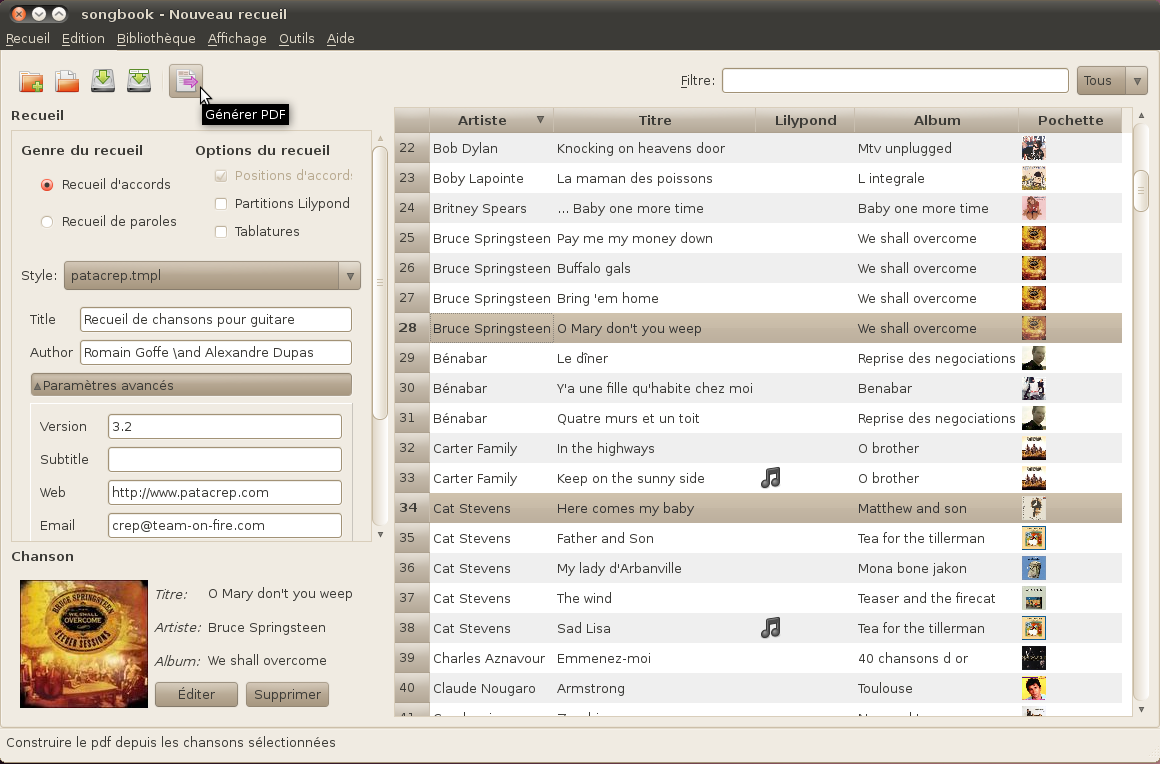
\includegraphics[width=\textwidth]{sbc-v0-3-01}
  \caption{Patacrep Songbook Client~: interface pour la génération de
    recueils de chansons.}
  \label{fig:sb-client}
\end{figure}

Pour lancer l'application, faites \Key{Alt}+\Key{F2}
\command{songbook-client} ou dans un terminal~:
\begin{unix}
  songbook-client
\end{unix}

Une fois l'application lancée, il est important~:
\begin{itemize}
\item d'indiquer le chemin du songbook dans les préférences (par
  exemple \directory{/home/user/songbook}). Ce répertoire devant impérativement
  contenir le makefile et le répertoire \directory{songs/} avec les chansons
  disponibles~;
\item de resynchroniser la base de données avec le nouveau répertoire
  indiqué (Fichier/Synchroniser).
\end{itemize}

\begin{nota}
  La synchronisation est à utiliser dès lors que vous modifiez le
  contenu du répertoire \directory{songs/} lorsque vous rajoutez un nouveau
  fichier (chanson, image) ou lorsque vous déplacez le répertoire
  \directory{songbook/}.  Il n'est pas nécessaire de synchroniser si vous
  avez simplement édité un fichier (correction, \dots\,).
\end{nota}

\subsection{La bibliothèque des chansons}

\subsection{L'éditeur de chansons}

%*******************************************************************************
\section{Générer un recueil}
%*******************************************************************************

\paragraph{Sélection des chansons}
Cliquez sur les chansons que vous souhaitez voir apparaitre dans votre
recueil.  Les chansons sélectionnées sont en surbrillance. Utilisez
l'action \Key{Générer PDF} pour générer le pdf disponble depuis le
menu Recueil/Générer ou depuis le bouton à droite dans la barre
d'outils.

\paragraph{Enregistrez votre recueil}
Un recueil est un fichier .sb dans lequel sera enregistré la liste des
chansons sélectionnées ainsi que les options et les champs
personnalisés du recueil lui-même.



%*******************************************************************************
\section{Ajouter une chanson}
%*******************************************************************************

\todo

%*******************************************************************************
\section{FAQ}
%*******************************************************************************

\paragraph{Comment signaler un bug ?}
Directement sur Github (\todo{url}) ou via le forum.

\paragraph{Erreur Sqlite au démarrage} 
Si vous voyez une boîte de dialogue d'avertissement se lancer au
démarrage de l'application indiquant que le support de sqlite est
nécessaire, vous ne pourrez pas utiliser l'interface. Vérifiez que
votre système dispose bien du support Qt de sqlite.

\paragraph{Les partitions de solfège n'apparaissent pas}
Si la compilation de votre recueil de chansons n'intègre pas les
partitions malgré l'option \emph{Lilypond} correctement cochée dans les
préférences, vérifiez que Lilypond est bien installé sur votre système. 

\paragraph{La bibliothèque des chansons est vide} 
Vérifiez que le chemin d'accès au patacrep songbook est correctement
renseigné dans Édition/Préférences.  Le chemin indiqué doit contenir
impérativement le makefile et le répertoire \directory{songs/}.

\paragraph{Erreurs après renommage/suppression d'une chanson} 
Un ``make clean'' ou, depuis l'interface, Recueil/Nettoyer devrait
régler le problème. S'il persiste encore, une solution radicale
consiste à supprimer manuellement tous les fichiers \ext{.d} présents
dans \directory{$\sim$/songbook}.

